\section{Tries}

\subsection{Preprocessing Strings}
\begin{itemize}
    \item Durch Vorverarbeitung des Musters wird eine Geschwindigkeitsverbesserung beim Suchen erzielt
    \item Nach Vorverarbeitung des Musters erzielt der KMP Algorithmus eine Geschwindigkeit, die proportional zur Text-Grösse ist
    \item Ist der Text gross, unveränderlich und wird oft durchsucht (z.B. das Werk von Shakespeare): man könnte anstelle des Musters den Text vorverarbeiten
    \item Trie ist eine kompakte Datenstruktur für die Repräsentation einer Menge von Strings, wie z.B alle Wörter eines Textes
    \item Tries erlauben Pattern Matching mit einer Geschwindigkeit welche proportional zur Grösse des Patterns ist
\end{itemize}


\subsection{Standard Tries}
für eine Menge von Strings S ist ein geordneter Baum, so dass:
\begin{itemize}
    \item jeder ausser dem Wurzel-Knoten ein Zeichen hat
    \item die Pfade von den externen Knoten zur Wurzel die Strings von S beinhalten
\end{itemize}
\vspace{-8pt}
\begin{center}
    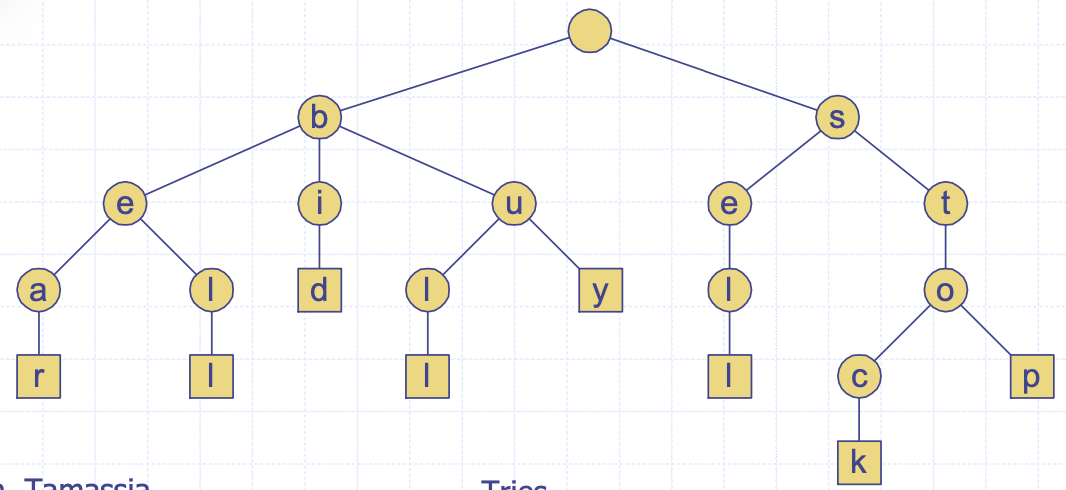
\includegraphics[scale=.3]{graphic/09 Tries/Standard Tries.png}
\end{center}
\vspace{-10pt}
\subsubsection{Laufzeit}
\begin{itemize}
    \item benötigt O(n) Speicher
    \item Suchen, Einfügen und Löschen in O(dm)
    \begin{itemize}
        \item n = totale Länge der Strings in S
        \item m = Länge des String-Parameters der Operation
        \item d = Grösse des Alphabets
    \end{itemize}
\end{itemize}
\subsubsection{Suche}
\begin{center}
    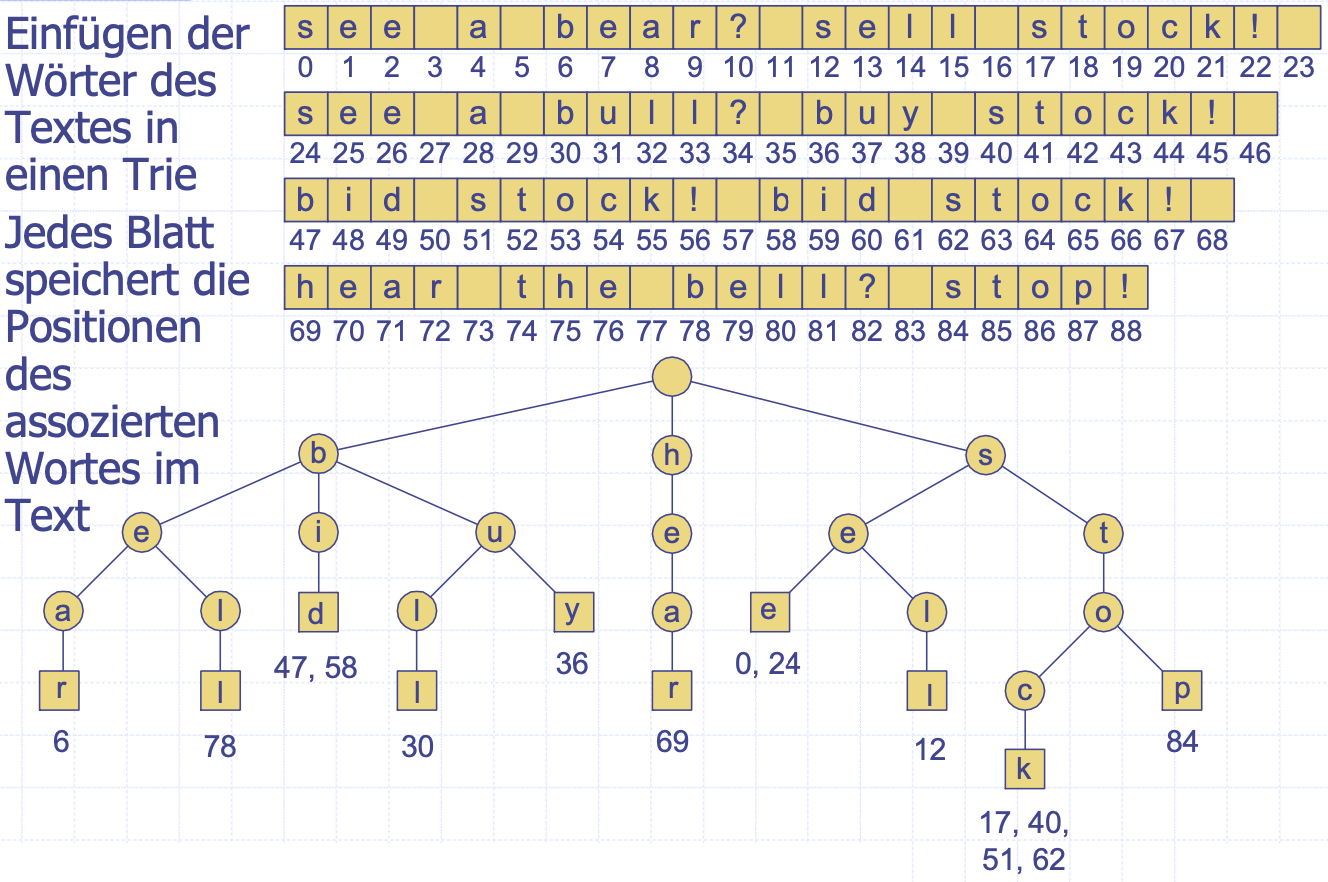
\includegraphics[scale=.25]{graphic/09 Tries/suche.png}
\end{center}
\vspace{-8pt}


\subsubsection{Komprimierte Tries}
\begin{itemize}
    \item wird von einem Standard-Trie hergeleitet
    \item Komprimierung von Pfaden von redundanten Knoten
\end{itemize}
\vspace{-8pt}
\begin{multicols}{2}
Standard-Trie:
\begin{center}
    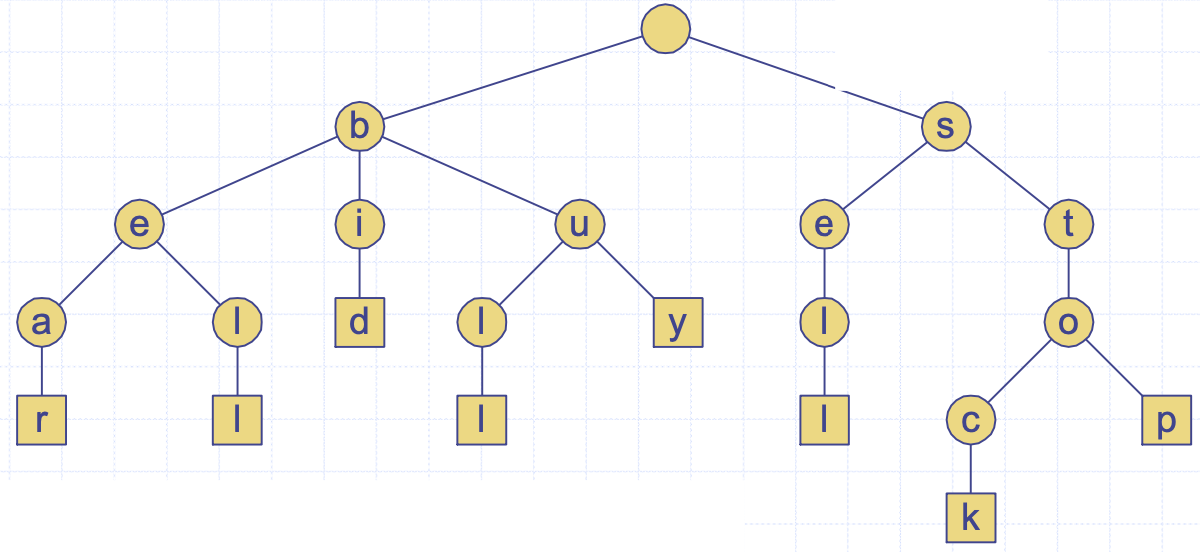
\includegraphics[scale=.165]{graphic/09 Tries/unkomprimiert.png}
\end{center}
    \columnbreak
Komprimierter Trie:
\begin{center}
    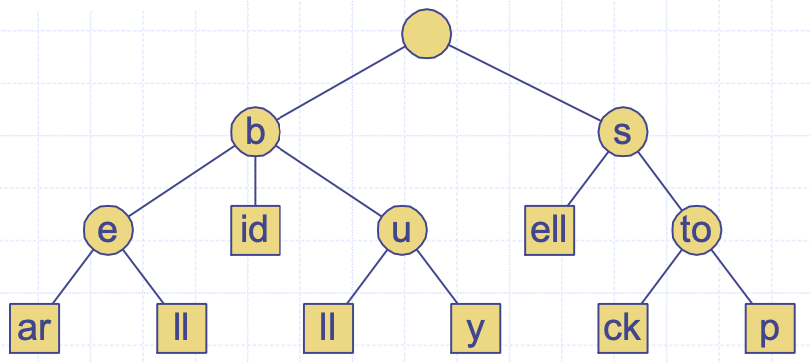
\includegraphics[scale=.23]{graphic/09 Tries/komprimiert.png}
\end{center}
\end{multicols}
\vspace{-8pt}
\subsubsection{Kompakte Repräsentation}
\begin{itemize}
    \item Knoten speichert Indizes anstelle von Substrings
    \item Benötigt O(s) Speicher, wobei s die Anzahl Strings im Array ist
    \item Dient als eine Hilfs-Index-Struktur
\end{itemize}
\vspace{-8pt}
\begin{center}
    \includegraphics[scale=0.28]{graphic/09 Tries/Kompakte_Repräsentation.png}
\end{center}
\vspace{-8pt}



\subsection{Suffix Trie}
\begin{itemize}
    \item Suffix-Trie eines Strings X ist der komprimierte Trie von allen Suffixen von X
\end{itemize}
\vspace{-8pt}
\begin{center}
    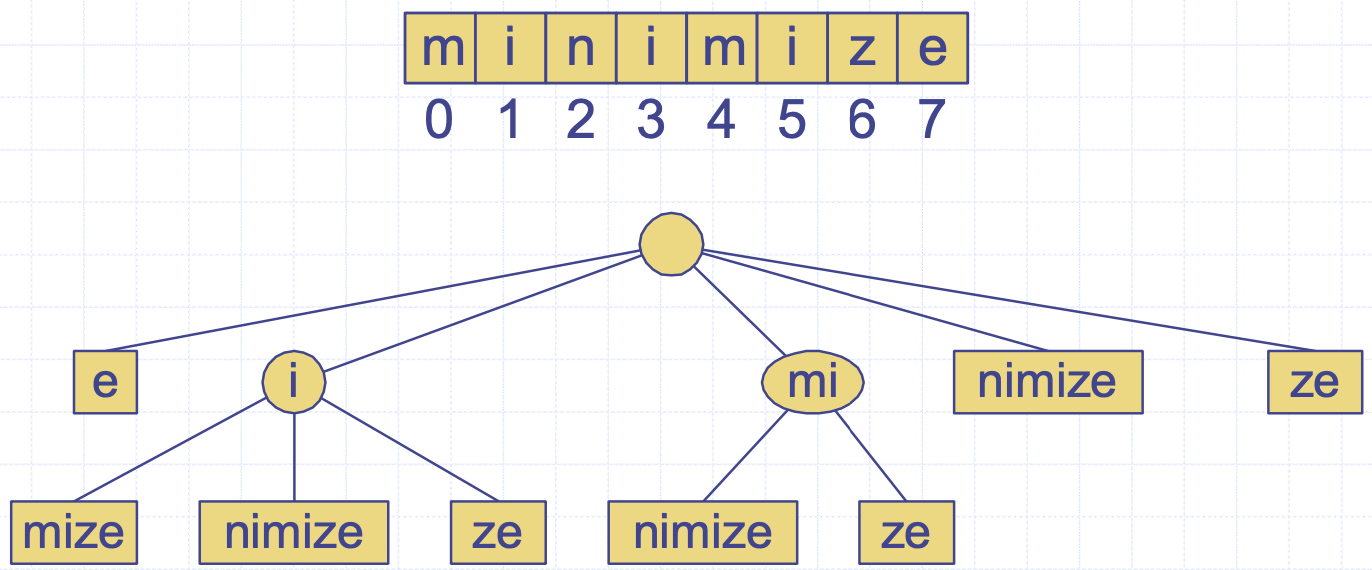
\includegraphics[scale=0.25]{graphic/09 Tries/Suffix.png}
\end{center}
\vspace{-8pt}
\subsubsection{Laufzeit}
\begin{itemize}
    \item benötigt O(n) Speicher
    \item Pattern Matching in X in O(dm)
    \item in O(n) Zeit erstellt werden
    \item X = Strings
    \item n = Länge von X
    \item d = Grösse des Alphabet
    \item m = Länge des Patterns
\end{itemize}

\vfill
$ $
\columnbreak



\newpage